\documentclass[10pt]{beamer}
\usetheme[
%%% option passed to the outer theme
%    progressstyle=fixedCircCnt,   % fixedCircCnt, movingCircCnt (moving is deault)
  ]{Feather}
\setbeamertemplate{navigation symbols}{}  
% If you want to change the colors of the various elements in the theme, edit and uncomment the following lines
\definecolor{blue}{rgb}{0.01, 0.28, 1.0}
% Change the bar colors:
%\setbeamercolor{Feather}{fg=blue!20,bg=blue}

% Change the color of the structural elements:
%\setbeamercolor{structure}{fg=red}

% Change the frame title text color:
%\setbeamercolor{frametitle}{fg=blue}
% Change the normal text color background:
%\setbeamercolor{normal text}{fg=black,bg=gray!10}
%-------------------------------------------------------
% INCLUDE PACKAGES
%-------------------------------------------------------

\usepackage[utf8]{inputenc}
\usepackage[english]{babel}
\usepackage[T1]{fontenc}
\usepackage{helvet}
\usepackage{svg}
\usepackage{minted}
\usepackage{dirtree}

%-------------------------------------------------------
% DEFFINING AND REDEFINING COMMANDS
%-------------------------------------------------------
\usepackage{xcolor}
\usepackage{listings}

\definecolor{mGreen}{rgb}{0,0.6,0}
\definecolor{mGray}{rgb}{0.5,0.5,0.5}
\definecolor{mPurple}{rgb}{0.58,0,0.82}
\definecolor{backgroundColour}{rgb}{0.95,0.95,0.92}

% colored hyperlinks
\newcommand{\chref}[2]{
  \href{#1}{{\usebeamercolor[bg]{Feather}#2}}
}

%-------------------------------------------------------
% INFORMATION IN THE TITLE PAGE
%-------------------------------------------------------

\title[Ansible] % [] is optional - is placed on the bottom of the sidebar on every slide
{ % is placed on the title page
      \textbf{Ansible:}
}

\subtitle[]
{
      \textbf{a Software Architecture Analysis}
}


\author[Simone Berni]
{     Presented by:\\ Simone Berni
}



%-------------------------------------------------------
% THE BODY OF THE PRESENTATION
%-------------------------------------------------------

\begin{document}

%-------------------------------------------------------
% THE TITLEPAGE
%-------------------------------------------------------

{\1% % this is the name of the PDF file for the background
\begin{frame}[plain,noframenumbering] % the plain option removes the header from the title page, noframenumbering removes the numbering of this frame only
  \titlepage % call the title page information from above
\end{frame}}
%Good morning everyone, my name is Simone Berni and my presentation is about Ansible




\begin{frame}[fragile]{What is Ansible?}
Ansible is an open-source IT automation engine.\\
Its main tasks are:
\begin{itemize}
    \item Hosts orchestration
    \item Application deployment
    \item Configuration management
    \item Cloud Provisioning
\end{itemize}
\end{frame}
%First of all, what is Ansible? Why someone wants to use this software?  4 are the  main goal of ansible: enable to orchestrate, inside a complex network, how the services behave and are connected to eachother. For example, if in my server I have apache, i want that Mysql is up too and at the latest version. Is used to deploy application, using the power of the Playbook, that we will see later, to describe the desired state of the system. Configuration management, again, is able to describe the exact configuration of one node in the system. Ansible is able to manage the provision of virtual and cloud machines. I don't know if someone you already know what provisioning of a virtual machine means, but for example I use Ansible during my security challenges because I want to have a virtual machine that has already some configuration, for example python must be the latest, must have already some tools installed, the packages are updates and so on. Since I do this a lot, i created an Ansible configuration to create it everytime.




\begin{frame}[fragile]{Utility tree}{Non functional requirements}
\begin{figure}
  \centering
  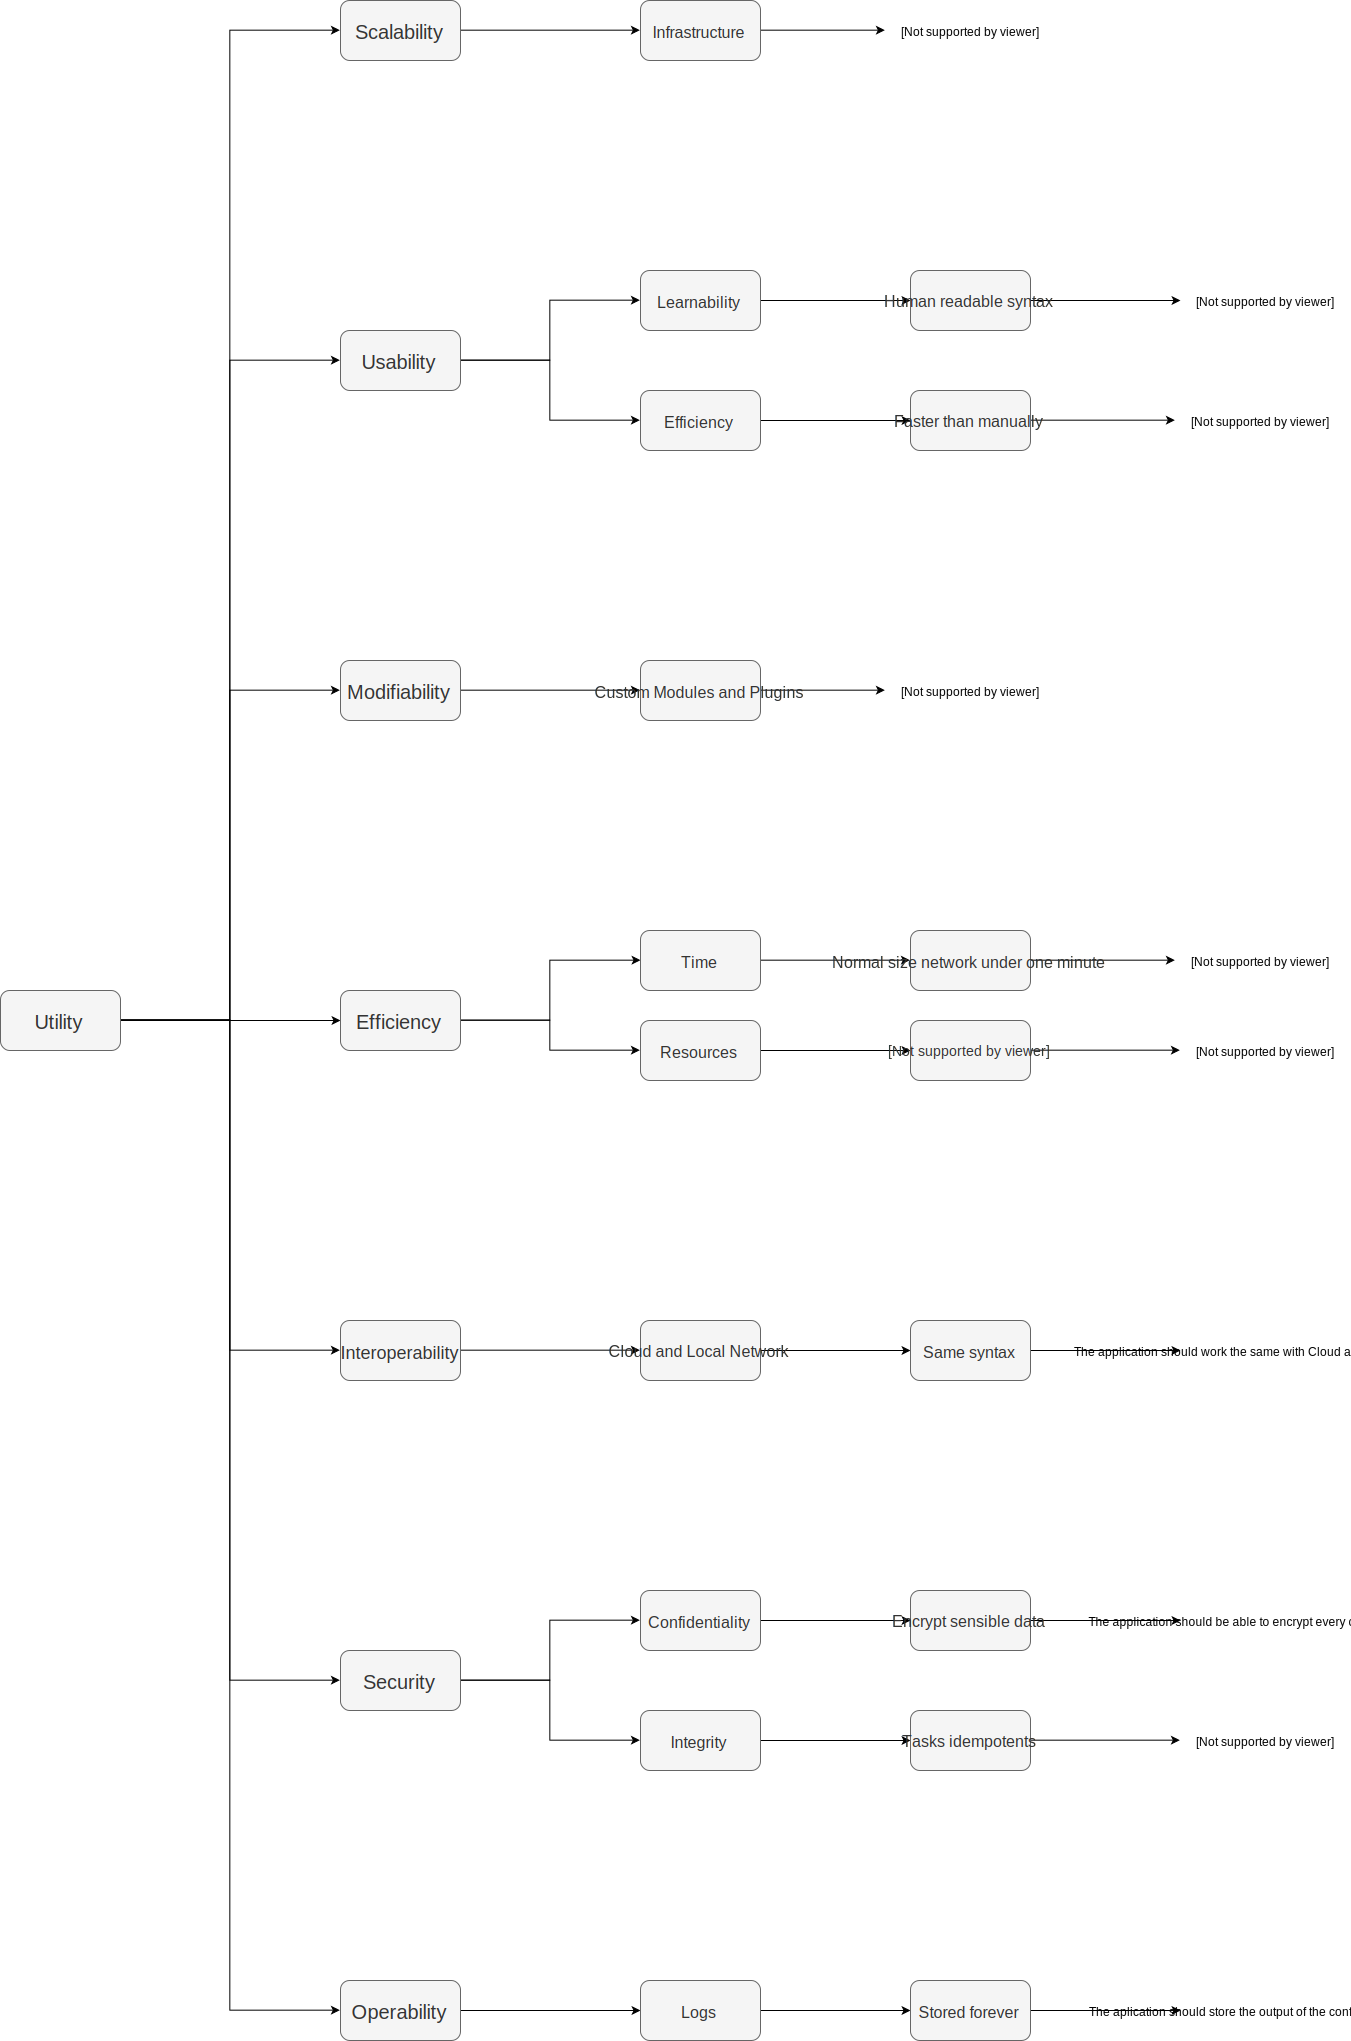
\includegraphics[width=0.45\textwidth]{UtilityTree.jpg}
\end{figure}
\end{frame}
%I gambled that the utility tree was visibile during the presentation: if it wasnt i had the use cases in another slide. 
%Scalability: Ansible must work with an high number of hosts. Why? Because is a giant limitation put a upperband of the network size. If the network will grow, ansible must be able to manage everynode
%Usability: we have 2 requirement, that it must be faster than doing so manually, otherwise no one will want to use Ansible because they can do it faster,and that its syntax must be human readable even from people without a programming background. This removes overhead to have to learn another language and the devops can start to configure from day0
%Modifability it must be possible to create custom modules if the builting are not enought
%Efficiency we have some upperband during the execution of ansible, because it must be faster than doing manually and it must be similar to its competitor, otherwise, again, no one would choose Ansible
%Interoperability is interesting: the world is going to cloud services, meaning that Ansible must work even with cloud machines. If we want to have a strong requirement is that for the engineer it must be transparent if we are working with a cloud or a common machine.
%Security in 2020 is pretty much a must. I want to connect to my machines in a secure way, SSH for example, and i want that the sensible data inside my configuration files is encrypted. Maybe because i want to put my files in a cloud machine, and i want to have another level of encryption. 
%Operability, is necessary to have some kind of logs of our system and since we will want to see the evolution of the system, the logs must be kept forever


\begin{frame}[fragile]{Use cases}
\resizebox{1\textwidth}{!}{%
\begin{tabular}{|p{0.6cm}|p{1.8cm}|p{5cm}|}
\hline
\textbf{Use Case} &\textbf{Description}&  \textbf{Scenario} \\
\hline
\hline
UC1 & Manage Users & Every node of the infrastructure has the same set of users and every user is able to log in every machine. \\
\hline
UC2 & Install Application & Every node of the infrastructure should be able to install the same software, even if the machines have different OS, packet manager and configurations. \\
\hline
UC3 & Provide reports & Whenever the nodes in the network are modified via Ansible, a report of what has be done, what was sucessfull and what not, has to be created.   \\
\hline
UC4 & History and Downgrade & For each node of the infrastructure the administrator has to be able to see its history and has to be able to downgrade the system to a previus version.\\
\hline

\hline
\end{tabular}
\quad
\begin{tabular}{|p{0.6cm}|p{1.8cm}|p{5cm}|}
\hline
\textbf{Use Case} &\textbf{Description}&  \textbf{Scenario} \\
\hline
\hline
UC5 & Configuration Syntax & The syntax has to be easy to remember and to understand, since the administrator wants to focus on what has to be done, not how to write it. 

\\

\hline
UC6 & Manage Cloud & The user should be able to use Anisble to manage many Amazon AWS instances. 

\\

\hline
UC7 & Extendable & If the builtin modules doesn't answer a user problem, should be easy to create and integrate a new custom module. 

\\

\hline
UC8 & Secure Connection & The sensible data should travel in a secure communication channel to the nodes.

\\

\hline
\end{tabular}
}
\end{frame}

\begin{frame}[fragile]{Non functional requirements}

\resizebox{1\textwidth}{!}{%
\begin{tabular}{|p{1cm}|p{2cm}|p{3cm}|p{1.8cm}|}
\hline
\textbf{Id} &  \textbf{Requirement} & \textbf{Scenario} & \textbf{Associated Use Cases} \\
\hline
\hline
NF1 & Usability & The application should be able to configure three nodes easier and faster than manually & UC1 \\
\hline
NF2 & Usability & The application should be able to configure any part of the system using the same syntax structure & UC1, UC2, UC5 \\
\hline
NF3 & Modifiability & The application should allow the creation of any kind of custom modules & UC7 \\
\hline
NF4 & Efficiency & The application should be able to configure a medium size network(15 nodes) in under 2 minute & UC6 \\
\hline
NF5 & Interoperability & The application should work the same with Cloud and company's network & UC6 \\
\hline

\hline
\end{tabular}
\quad
\begin{tabular}{|p{1cm}|p{2cm}|p{3cm}|p{1.8cm}|}
\hline
\textbf{Id} &  \textbf{Requirement} & \textbf{Scenario} & \textbf{Associated Use Cases} \\
\hline
\hline
NF6 & Security & The application should be able to connect to the hosts via SSH & UC8 \\
\hline
NF7 & Security & The application should be able to encrypt sensible data in a secure way & UC8 \\
\hline
NF8 & Operability & The application should store the history for each node forever & UC4\\
\hline
NF9 & Scalability & The application should work with at least 50 nodes without losing performance & UC2, UC6 \\
\hline
\end{tabular}
}
\end{frame}
%Come prima solo spezzettato








\begin{frame}[fragile]{Structures}

\begin{center}
\includegraphics[width=1\textwidth]{Schema.jpg}
\\
\textit{The Playbook is like an instruction manual, where the Inventory is the material, the Modules are the tools and the Vault the cabinet}
\end{center}
\end{frame}
%Ok, let's see how the structure works for Ansible: the main component is the Command Center, that is the computer where Ansible lies. The hosts machines are the nodes in our network that we wants to configure and that are accessibile to the end users.
%For doing the communication, ansible connect from the CC to the hosts via SSH: in thi way there is the guarranty that no middle man are hijacking the conversation. 
%Ansible is constructed of many pieces that works together: and that metaphor really do the job of explaining how they are related. The devops creates an Inventory, grouping the nodes that have to be managed. After that he secure the sensible data inside the inventory with the Vault, that encrypt it. Now is time to the execution of tasks: inside the playbook are defined what are we going to do, the modules is how this is done and the plugin what must be done on the CC to enable that.
%Let's see in the details each structure



\begin{frame}[fragile]{Structures}{Inventory}
\begin{itemize}
    \item List or groups of hosts that Ansible will work against
    \item Can be used to assign value to variables and to create aliases 
    \item Is possible to create a filesystem grouping many inventory files
\end{itemize}
\end{frame}
%Like i said the main goal of the inventory component is to list and groups the hosts that Ansible will work against
%But has many secondaries uses like for example it can be used to assign value to variables, or create alias that will be used inside the playbook.
%In a complex network the relations between the hosts will be complex. For having everything under control, the inventory is commonly splitted in many files creating a real filesystem that ansible will manage.
%Words sometimes are not enought for understand how things works, and I believe that examples are more powerfull: this is why we have an example for each structure that explains how to use it



\begin{frame}[fragile]{Structures}{Inventory - Example}
\begin{minipage}[t]{0.45\linewidth}


\begin{minted}[
  ]{yaml}
[dbservers]
db01.test.example.com
db02.test.example.com

[appservers]
app01.test.example.com
app02.test.example.com
app03.test.example.com
  \end{minted}
\footnotesize \textit{Inventory example}
\end{minipage}
%
\begin{minipage}[t]{0.45\linewidth}

  \dirtree{%
  .1 /etc/ansible/.
  .2 hosts.
  .2 hosts\_var/.
  .3 DisiLab.
  .2 group\_vars/.
  .3 web\_servers.
  .3 datacenters.
  .3 \vdots.
  }
  \footnotesize \textit{Inventory filesystem example}
\end{minipage}

\end{frame}
%Here for example we have create 2 groups: the db servers and the app servers. Having listed them in one group, after that when we want to execute a task, we will just run it against the group, and Ansible will manage the single hosts that are in the group.
%The second example explains a easy sub filesystem for manage many hosts. For example inside DisiLab there are the alias with each IP and a name, enumerating the hosts, and in the group\_vars directory there are file for each group that will be managed
%Again, nothing complex, is always easy to understand the structure because Ansible has to be fast to deploy.


\begin{frame}[fragile]{Structures}{Module}
\begin{itemize}
    \item A small program that is executed on each host
    \item It describes the desired state of the system
    \item Has to be idempotent
    \item The output can be \textit{ok}, \textit{changed}, \textit{failed}
    \item It is used inside a Playbook
    \item Is possible to create custom modules
\end{itemize}
\end{frame}
%Remember that modules are the tools, they do the taks. They are just small programs, that can be write in any language, that must return a json. The return value can be ok, if the tasks was successfull, changed if it had to modify sometyhing on the system, failed if failed. They have to be idempotent, meaning that runs many times the same module doesn't have to produce effects. This is done just checking if the system is already in the desired state. In fact, when configuring a module to use it, you describe how the system will be. Another important thing is that you can create custom modules, if no one of the bultin satisfies your needs. It just needs to respect the costraints said before. You can use a module in 2 way: the standard way, inside a playbook, or via command line if you just need something faster. The first choice is what is normally used, because you want to orchestrate a system.
%Again an example


\begin{frame}[fragile]{Structures}{Module - Example}
\begin{minipage}[t]{0.45\linewidth}


\begin{minted}[
  ]{yaml}
name: restart webserver
    service:
      name: httpd
      state: restarted
  \end{minted}
\footnotesize \textit{Module service example}
\end{minipage}
%
\begin{minipage}[t]{0.45\linewidth}


\begin{minted}[
  ]{yaml}
name: write apache config
    template:
      src: /srv/httpd.j2
      dest: /etc/httpd.conf
  \end{minted}
\footnotesize \textit{Module template example}
\end{minipage}
\end{frame}
%There are the 2 modules inside a playbook. The first is the module service, that manages the state of a service inside a host, the second is the module template, that is used to move, create and edit files


\begin{frame}[fragile]{Structures}{Vault}
\begin{itemize}
    \item Manages the encryption and decryption of sensible data
    \item Can encrypt every Ansible file
    \item Is possible to have variable-level encrpytion
    \item The unlocking password can be inserted via prompt or password manager
\end{itemize}
\end{frame}
%The vault is used to encrypt things. Is completely transparent to the engineer, Ansible will decrypt automatically the content and parse it like if it wasnt encrypted, it just asks for the key like pass or a common password manager. The vault can encrypt at 2 levels: or the entire file, meaning that everything inside will be gibberish for a not authenticated user, or just the sensible data, for example a password, and let the rest of the file be decrypted. In this way is more easy to let third party see the configuration and give advices, and critics, or just evaluate the configuration job without revealing sensible data


\begin{frame}[fragile]{Structures}{Playbook}

\begin{itemize}
    \item Is a list of play, or tasks, that must be done against some hosts
    \item Enable the possibility to logically group tasks
    \item Yaml Syntax
    \item Must be idempotent
    \item Supports \textit{Jinja2} templating
    \item Enable the possibility to retrieve \textit{facts}
    \item Supports conditionals and loops
\end{itemize}
\end{frame}
%The core of Ansible, the playbook. Is a very simple idea, but powerfull: is a list of tasks that has to be done on some group of hosts. That's it. That's ansible. That's the power of this architecture. In a moment we will see an example and it will be clearer. Since each module must be idempotent, even the final playbook, that is a composition of tasks, will be idempotent. This way a playbook can be run an infinite number of times without creating issues. Ansible is built on top of Python, and like many other softwares built over Python uses Jinja2 templating. An example or a common one is Flask, for web development, i dont know if some one you know it. The templating system enable to configure commands runtime. Another thing that ansible can retrieve is Facts about your networks and hosts. For example you want to execute something only if the OS is Arch. You can ask Ansible to retrieve information about the host, anche check if the value of OS is arch. If so do something. This is possible with the use of conditionals and loops, that Ansile has enabled inside a playbook. This was done because, many times, you want to do X if Y was installed, otherwise do Z. Or you want to move N files, and so on.

\begin{frame}[fragile]{Structures}{Playbook - Example}
\begin{minipage}[t]{0.45\linewidth}
\begin{minted}[
  ]{yaml}
---
hosts: webservers
remote_user: root
tasks:
  name: apache latest
  yum:
    name: httpd
    state: latest
  name: apache config 
  template:
    src: /srv/httpd.j2
    dest: /etc/httpd.conf
\end{minted}
\footnotesize \textit{Playbook example}
\end{minipage}
%
\begin{minipage}[t]{0.45\linewidth}
\begin{minted}[
  ]{yaml}
---
hosts: webservers
remote_user: root
tasks:
  name: apache latest
  yum:
    name: httpd
    state: latest
  name: apache config
  template:
    src: "{{local_path}}}httpd.j2"
    dest: "{{remote_path}}httpd.conf"

  \end{minted}
\footnotesize \textit{Playbook jinja2 example}
\end{minipage}
\end{frame}
%YUM is a packet manager for CentOS if i remember correctly,


\begin{frame}[fragile]{Structures}{Plugin}
\begin{itemize}
    \item Pieces of code that augment Ansible's core functionality
    \item The code is normally executed on the control machine, not on the hosts
    \item Many are shipped with Ansible
    \item Is possible to create custom plugins
    \item Example: Connection plugin
\end{itemize}
\end{frame}
%The plugins are used to extend Ansible core functionalities. For example the Connection plugin is used to decide how the command center connect to each hosts. They are similar to the modules, just for the fact the normally they are run on the CC instead of hosts. Many are shipped with Ansible, but is possible to create custom ones, like the modules. There are more constraint that must be respected tho: they must be wrote in Python, they must return a JSON file, return string as unicode and raise errors. Nothing strange, just a little formality to be able to connect to rest of Ansible.

\begin{frame}[fragile]{Functions}
\resizebox{1\textwidth}{!}{%
\begin{tabular}{|p{1.6cm}|p{1.8cm}|p{4cm}|}
\hline
\textbf{Req} &\textbf{Component}&  \textbf{Description} \\
\hline
\hline
Usability   Efficiency & Module & Ansible offers enough modules to complete every task that the user need to accomplish on the remote machines with just one Yaml line.\\
\hline
Usability   Syntax & Playbook & Ansible uses Yaml syntax, and each play has the same structure and syntax, but different keys and values.\\
\hline
Modifiability & Module and Plugin & Ansible offers the possibility to create new modules and plugins that must return JSON data.\\
\hline
Scalability & Inventory and Playbook & Using Ansible's inventory is possible to group hosts together and to run the same task to every host sequentially.\\
\hline

\hline
\end{tabular}
\quad
\begin{tabular}{|p{1.6cm}|p{1.8cm}|p{4cm}|}
\hline
\textbf{Req} &\textbf{Component}&  \textbf{Description} \\
\hline
\hline
Inter-operability & Module & For the devops engineer, Ansible works exactly the same with Cloud and local hosts, but has to use differents modules to accomplish the same result.\\
\hline
Security  Connection & Module & SSH is the default way to execute task.

\\
\hline
Security  Encryption & Vault & The vault utility offers the possibility to encrypt files without reducity the Ansible power.

\\
\hline
Operability   History & Plugin & The plugin \textit{log\_plays} will save the Playbook log to a file, but is a devops engineer task to preserve them in a solid way.

\\
\hline
\end{tabular}
}
\end{frame}




\begin{frame}[fragile]{Behaviour}{Work flow}
\begin{center}
\includegraphics[width=0.50\textwidth]{Flow.png}
\end{center}
\end{frame}
%

%
%\begin{frame}[fragile]{Rationale}{Why?}
%\begin{itemize}
%    \item Simple architecture $\rightarrow$ \textit{Fast deploy}
%    \item Modularity $\rightarrow$ \textit{Customizable}
%    \item YAML $\rightarrow$ \textit{Simple to remember}
%    \item Python $\rightarrow$ \textit{Emerging and powerfull language}
%    \item Vault $\rightarrow$ \textit{Encryption is a must}
%    \item Inventory $\rightarrow$ \textit{Organize nodes for roles}
%    \item Playbook $\rightarrow$ \textit{Organize tasks}
%\end{itemize}
%\end{frame}
%First of all we have to load the plugins, this is done by the plugin loader that will consider each plugin as a python object. After that we have to retrieve the information from the inventory, this is done first by decrypting it using the vault, and than parsing via a YAML parser. Thi can be retrieve an error, if the syntax is wrong, or go on with the next phase. We have to parse the playbook, again it uses a YAML syntax, and then execute the playbook, connecting via SSH to each host and retrieving the output


\begin{frame}[fragile]{Critical Analysis}{Pros}
\begin{itemize}
    \item \textbf{Easy to learn}: clear documentation full of examples
    \item \textbf{Agentless}: fast deploy on every node
    \item \textbf{Yaml syntax}: human readable, without having to remember a complex keywords or an ad hoc syntax
    \item \textbf{Opensource}: the source code is available to everyone
     \item \textbf{Python}: the fastest growing language nowadays
\end{itemize}
\end{frame}



\begin{frame}[fragile]{Critical Analysis}{Cons}
\begin{itemize}
    \item \textbf{CLI only}: designed to be configurable from its prefered text editor, an attempted has beed made with Ansible Tower
    \item \textbf{Young}: is the most recently developed orchestration tool, and inevitably bugs could occur
    \item \textbf{SSH}: modules execution relie completely on SSH 
\end{itemize}
\end{frame}
%SSH can be a problem for many reasons: first of all if the SSH connection is bad, or iptables are not configured, and so on, is a single point of failure. If ssh crash, then the executions fails. Another problem is how is used ssh: technically we must do 3 connections for each node: the first create a temporary folder, the secondo move the files and the third executes the files. Is possible to use a technic called pipeling, with just one SSH connection that opens python in the host machine and than it pipeline inside the modules that must be executed.


\begin{frame}[fragile]{Similar Architectures}
\begin{itemize}
    \item \textbf{Chef}
    \item \textbf{Puppet}
    \item \textbf{Saltstack}
\end{itemize}
\end{frame}


\begin{frame}[fragile]{Similar Architectures}{Chef}
\begin{itemize}
    \item Architecture: \textbf{Master-agent}
    \item Fault tollerance: \textbf{Backup server}
    \item Language: \textbf{Ruby DSL}
    \item OS:\textbf{ Master Unix, Clients whatever}
\end{itemize}
\end{frame}


\begin{frame}[fragile]{Similar Architectures}{Puppet}
\begin{itemize}
    \item Architecture: \textbf{Master-agent}
    \item Fault tollerance:\textbf{ Multi master}
    \item Language: \textbf{Puppet DSL}
    \item OS: \textbf{Master Unix, Clients whatever}
\end{itemize}
\end{frame}



\begin{frame}[fragile]{Similar Architectures}{OpenStack}
\begin{itemize}
    \item Architecture: \textbf{Master-agent}
    \item Fault tollerance: \textbf{Can be Multi master}
    \item Language: \textbf{YAML}
    \item OS: \textbf{Master Unix, Clients whatever}
\end{itemize}
\end{frame}

\begin{frame}[fragile]{Conclusions}
Ansible is built with a proper design in mind: no overhead.  For this reason it doesn't support daemons, it uses YAML, the execution is via SSH and is only configurable using the prefered text editor. \\
This may create some issues, but the pros outweight the cons.
\end{frame}

{\1
\begin{frame}{References}
\fontsize{7}{9}\ttfamily
P.Masek, M. Stusek, J. Krejci, K. Zeman, J. Pokorny, M. Kudlacek, ''Unleashing Full Potential of Ansible Framework: University Labs Administration'', IEEE, Jyvaskyla, Finland, 5-18 May 2018, [2018 22nd Conference of Open Innovations Association (FRUCT)].\\
W. Yiran, Z. Tongyang, G. Yidong, ''Design and implementation of continuous integration scheme based on Jenkins and Ansible'', IEEE, Chengdu, China, 26-28 May 2018, [2018 International Conference on Artificial Intelligence and Big Data (ICAIBD)].\\
N. K. Singh, S. Thakur, H. Chaurasiya, H. Nagdev, ''Automated provisioning of application in IAAS cloud using Ansible configuration management'', IEEE, Dehradun, India, 4-5 Sept. 2015, [2015 1st International Conference on Next Generation Computing Technologies (NGCT)].\\
V. Shvetcova, O. Borisenko, M. Polischuk,''Domain-Specific Language for Infrastructure as Code'', IEEE, Velikiy Novgorod, Russia, 13-14 Sept. 2019, [2019 Ivannikov Memorial Workshop (IVMEM)].\\
J. Keating, ''Mastering Ansible'', Packt Publishing Ltd., Birmingham, Nov. 2015, pp 1-33.\\
"Ansible Documentation", Accessed on: Nov. 25, 2019, [Online], Avaible: \href{https://docs.ansible.com/ansible/latest/index.html}{https://docs.ansible.com/ansible/latest/index.html}

\end{frame}
}
 \end{document}